\section{Fundamentals}

\subsection{Python}
Python is a high-level, interpreted programming language known for its simplicity and readability. It was created by Guido van Rossum and first released in 1991. Python's design philosophy emphasizes code readability and productivity, making it an ideal language for both beginners and experienced programmers alike.

\subsubsection{Versions}
Python 2 and Python 3 represent two major versions of the Python programming language. Python 2, released in 2000, served as the primary version for many years until its end of life in 2020. Python 3, introduced in 2008, addressed design flaws and inconsistencies present in Python 2. Python 3 is actively maintained and recommended for all new projects, while Python 2 is no longer officially supported.

\subsubsection{Hello World}
This Python code will print "Hello, World!" to the console when executed. It's a simple yet classic introductory example often used to demonstrate the basic syntax of a programming language.

\begin{codebox}
\begin{minted}{python}
# Hello World Program
print("Hello, World!")
\end{minted}
\end{codebox}

\begin{itemize}
    \item \textbf{\# Hello World Program}: This line is a comment. It's meant to provide a brief description or title for the program. It does not affect the execution of the code but helps other developers understand the purpose of the program.
    \item \textbf{print("Hello, World!"):} This line is the actual Python code. It prints the string "Hello, World!" to the console. The \texttt{print()} function is used to display output.
\end{itemize}

\subsubsection{Official Python Documentation}
The official Python documentation is hosted online at \href{https://docs.python.org/3/}{docs.python.org}. It serves as the primary source of documentation for the Python programming language and its standard library.

\subsubsection{Applications}
Python is a versatile programming language widely used across various domains due to its simplicity, readability, and extensive libraries.
\begin{itemize}
    \item \textbf{Web Development}: Widely used for web development, with frameworks like Django and Flask for building web applications, APIs, and dynamic websites.
    \item \textbf{Data Science and Machine Learning}: Popular choice for data analysis, machine learning, and artificial intelligence projects, thanks to libraries like NumPy, pandas, scikit-learn, TensorFlow, and PyTorch.
    \item \textbf{Automation and Scripting}: Commonly used for automation tasks, scripting, and system administration, thanks to its ease of use and cross-platform compatibility.
    \item \textbf{Scientific Computing}: Used in scientific computing and computational modeling, with libraries like SciPy and Matplotlib for numerical calculations, data visualization, and plotting.
\end{itemize}

\newpage
\subsection{Data Types}

There are several built-in data types that are fundamental to the language's core functionality. Here's a brief overview of the main Python data types:

\subsubsection{Numeric Types}
\begin{codebox}
\begin{minted}{python}
my_int: int = 10
my_float: float = 3.14
my_complex: complex = 2 + 3j
\end{minted}
\end{codebox}
\begin{itemize}
\item \textbf{Integer}: Integer numbers, representing whole numbers
\item \textbf{Float}: Floating-point numbers
\item \textbf{Complex}: Complex numbers with a real and imaginary part
\end{itemize}

\subsubsection{Strings}
\begin{codebox}
\begin{minted}{python}
first_string: str = "Hello, World!"
second_string: str = 'Hello, World!'
\end{minted}
\end{codebox}
\begin{itemize}
\item \textbf{String}: Sequences of Unicode characters, immutable, enclosed in single or double quotes
\end{itemize}

\subsubsection{Collections}
A collection is a single variable used to store multiple values.
\begin{codebox}
\begin{minted}{python}
my_list: list[int] = [1, 2, 3, 4, 5]
my_tuple: tuple[int] = (1, 2, 3)
my_set: set[int] = {1, 2, 3}
my_frozenset: frozenset[int] = frozenset({1, 2, 3})
\end{minted}
\end{codebox}
\begin{itemize}
\item \textbf{List = []}: Ordered collection of items, mutable, duplicates are ok
\item \textbf{Tuple = ()}: Ordered collection of items, immutable, duplicates are ok
\item \textbf{Set = \{\}}: Unordered collection of unique items, mutable (add/remove items), no duplicates
\item \textbf{Frozenset = frozenset(\{\})}: Immutable version of a set
\end{itemize}

%\subsubsection{Dictionary}
\begin{codebox}
\begin{minted}{python}
my_dict: dict[str, int or str] = {
    "name": "John",
    "age": 30,
    "city": "New York"
}
\end{minted}
\end{codebox}
\begin{itemize}
\item \textbf{Dictionary}: Collection of key-value pairs, mutable and unordered collection
\end{itemize}

\subsubsection{Boolean Type}
\begin{codebox}
\begin{minted}{python}
my_boolean: bool = True  # Boolean value
\end{minted}
\end{codebox}
\begin{itemize}
\item \textbf{Boolean}: Represents truth values \texttt{True} or \texttt{False}.
\end{itemize}

\subsubsection{None Type}
\begin{codebox}
\begin{minted}{python}
my_none = None
\end{minted}
\end{codebox}
\begin{itemize}
\item \textbf{NoneType}: Represents the absence of a value or null value.
\end{itemize}

These are the primary built-in data types. Understanding these data types and their properties is essential for effective programming. Additionally, Python's dynamic typing system allows variables to change types dynamically, enhancing flexibility and ease of use.

\subsubsection{Comparison of List, Tuple, and Set}

\begin{table}[htbp]
\centering
\label{tab:comparison}
\begin{tabular}{|l|c|c|c|}
\hline
\textbf{Property} & \textbf{List} & \textbf{Tuple} & \textbf{Set} \\
\hline
\textbf{Creation} & \texttt{my\_list = [1,2,3]} & \texttt{my\_tuple = (1,2,3)} & \texttt{my\_set = \{1,2,3\}} \\
\hline
\multirow{2}{*}{\textbf{Ordering}} & Ordered & Ordered & Unordered \\
 & (Maintains insertion order) & (Maintains insertion order) & (No guaranteed order) \\
\hline
\multirow{2}{*}{\textbf{Duplicates}} & Allows & Allows & No duplicates \\
 &  &  & (Collection of unique elements) \\
\hline
\textbf{Mutability} & Mutable & Immutable & Mutable \\
\hline
\multirow{2}{*}{\textbf{Access Time}} & O(1) & O(1) & O(1) \\
 & (Constant time) & (Faster than list) & (Faster than list or tuple) \\
\hline
\end{tabular}
\end{table} 

\subsubsection{Dictionaries}
A dictionary is a built-in data type that allows you to store a collection of key-value pairs. It's a highly flexible data structure that provides efficient lookups, insertions, and deletions.

\begin{itemize}
    \item \textbf{Key}: Each key in a dictionary must be unique and immutable (such as strings, numbers, or tuples). Keys are used to access the corresponding values.
    \item \textbf{Value}: The associated value for each key in the dictionary. Values can be of any data type, including lists, tuples, dictionaries, or even other dictionaries.
\end{itemize}

A value in a dictionary can be checked using the \texttt{in} operator. However, by default, the \texttt{in} operator checks for keys in the dictionary, not values. To check if a value exists in a dictionary, the \texttt{values()} method can be utilized to obtain a view of the dictionary's values.

\begin{codebox}
\begin{minted}{python}
phonebook = {"Alice": "123456", "Bob": "789012", "Charlie": "345678"}

if "Bob" in phonebook:
    print("Bob's number is:", phonebook["Bob"])
else:
    print("Bob is not in the phonebook.")


if "345678" in phonebook.values():
    print("The number 345678 exists in the phonebook.")
\end{minted}
\end{codebox}

\newpage
\subsubsection{Type Conversion Methods}

Type conversion methods are functions or operations used to convert data from one type to another. These methods allow you to change the data type of a variable or value.

\begin{itemize}
    \item \texttt{int()}: Converts a value to an integer.
    \item \texttt{float()}: Converts a value to a floating-point number.
    \item \texttt{str()}: Converts a value to a string.
    \item \texttt{list()}: Converts an iterable to a list.
    \item \texttt{tuple()}: Converts an iterable to a tuple.
    \item \texttt{set()}: Converts an iterable to a set.
    \item \texttt{bool()}: Converts a value to a boolean.
\end{itemize}

These type conversion methods are essential for manipulating and transforming data between different types as needed in various programming scenarios. 

\subsubsection{List Comprehension}
List comprehension is a concise way to create lists. It allows to generate lists based on existing iterables such as lists, strings, or range objects, with a compact and readable syntax.

\begin{codebox}
\begin{minted}{python}
squares = [x**2 for x in range(10)]
print(squares)
# Output: [0, 1, 4, 9, 16, 25, 36, 49, 64, 81]
\end{minted}
\end{codebox}

\begin{codebox}
\begin{minted}{python}
numbers = [1, 2, 3, 4, 5, 6, 7, 8, 9, 10]
even_numbers = [x for x in numbers if x % 2 == 0]
print(even_numbers)
# Output: [2, 4, 6, 8, 10]
\end{minted}
\end{codebox}

\begin{codebox}
\begin{minted}{python}
# Define the dimensions of the matrix
rows = 3
columns = 3

# Create a 2D array (matrix) using list comprehension
matrix = [[0 for _ in range(columns)] for _ in range(rows)]
\end{minted}
\end{codebox}

\newpage

\subsection{Modules, Packages, and Namespaces}
\begin{itemize}
\item \textbf{Modules}\\
Individual files containing Python code, such as functions, classes, and variables. They allow you to organize your code into separate files for better maintainability and reusability. You can import modules in other scripts to use the code they contain.

\item \textbf{Packages}\\
Directories containing one or more modules and an \texttt{\_\_init\_\_.py} file. They provide a way to organize modules into a hierarchical structure. Packages allow you to manage larger projects more effectively by grouping related functionality together. You can import packages in your scripts to access the modules and their contents.

\item \textbf{Namespace}\\
Namespaces are closely related to modules and packages. Each module and package has its own namespace, which serves as a container for the names defined within it. This ensures that names defined in one module or package do not clash with names in another module or package. When you import the \texttt{math} module as \texttt{m}, you're creating a namespace \texttt{m} which contains all the names defined in the \texttt{math} module.
\end{itemize}

\begin{codebox}
\begin{minted}{python}
# Importing my_module from my_package
from my_package import my_module

# Importing math module
import math

# Using constants and functions from math module
print("The value of pi is:", math.pi)
print("The square root of 16 is:", math.sqrt(16))

# Using a function from my_module
my_module.say_hello()
\end{minted}
\end{codebox}

\subsubsection{Order of imports}
PEP 8 suggests a specific order to import different types of modules:
\begin{enumerate}
    \item Standard library imports
    \item Related third-party imports
    \item Local application or library-specific imports
\end{enumerate}

\subsubsection{The \texttt{\_\_name\_\_} Variable}
When Python runs a script, it sets the special variable \texttt{\_\_name\_\_} to "\_\_main\_\_" for the script that is being executed directly. If the script is imported as a module into another script, then \texttt{\_\_name\_\_} is set to the name of the module.

\begin{codebox}
\begin{minted}{python}
if __name__ == "__main__":
    # This code block will only run if the script is executed directly
    # It won't run if the script is imported as a module into another script
\end{minted}
\end{codebox}

%By utilizing the condition if \texttt{\_\_name\_\_ == "\_\_main\_\_":}, the code that is intended to execute solely when the script is directly executed can be distinguished from the code designed to run when the script is imported as a module. This separation ensures that specific sections of the script are executed appropriately based on how the script is invoked.

\newpage
\subsection{Built-in Functions}
The Python interpreter has a number of functions and types built into it that are always available. They are listed and described \href{https://docs.python.org/3/library/functions.html}{here} in alphabetical order.\\

Built-in functions are functions that are available in the Python interpreter without the need to import any external modules. They are part of the core Python language and provide basic functionality that is commonly used in programming tasks. Built-in functions span a wide range of operations, from basic arithmetic and type conversion to more specialized tasks like input/output operations and data manipulation.

\begin{figure}[h!]
    \centering
    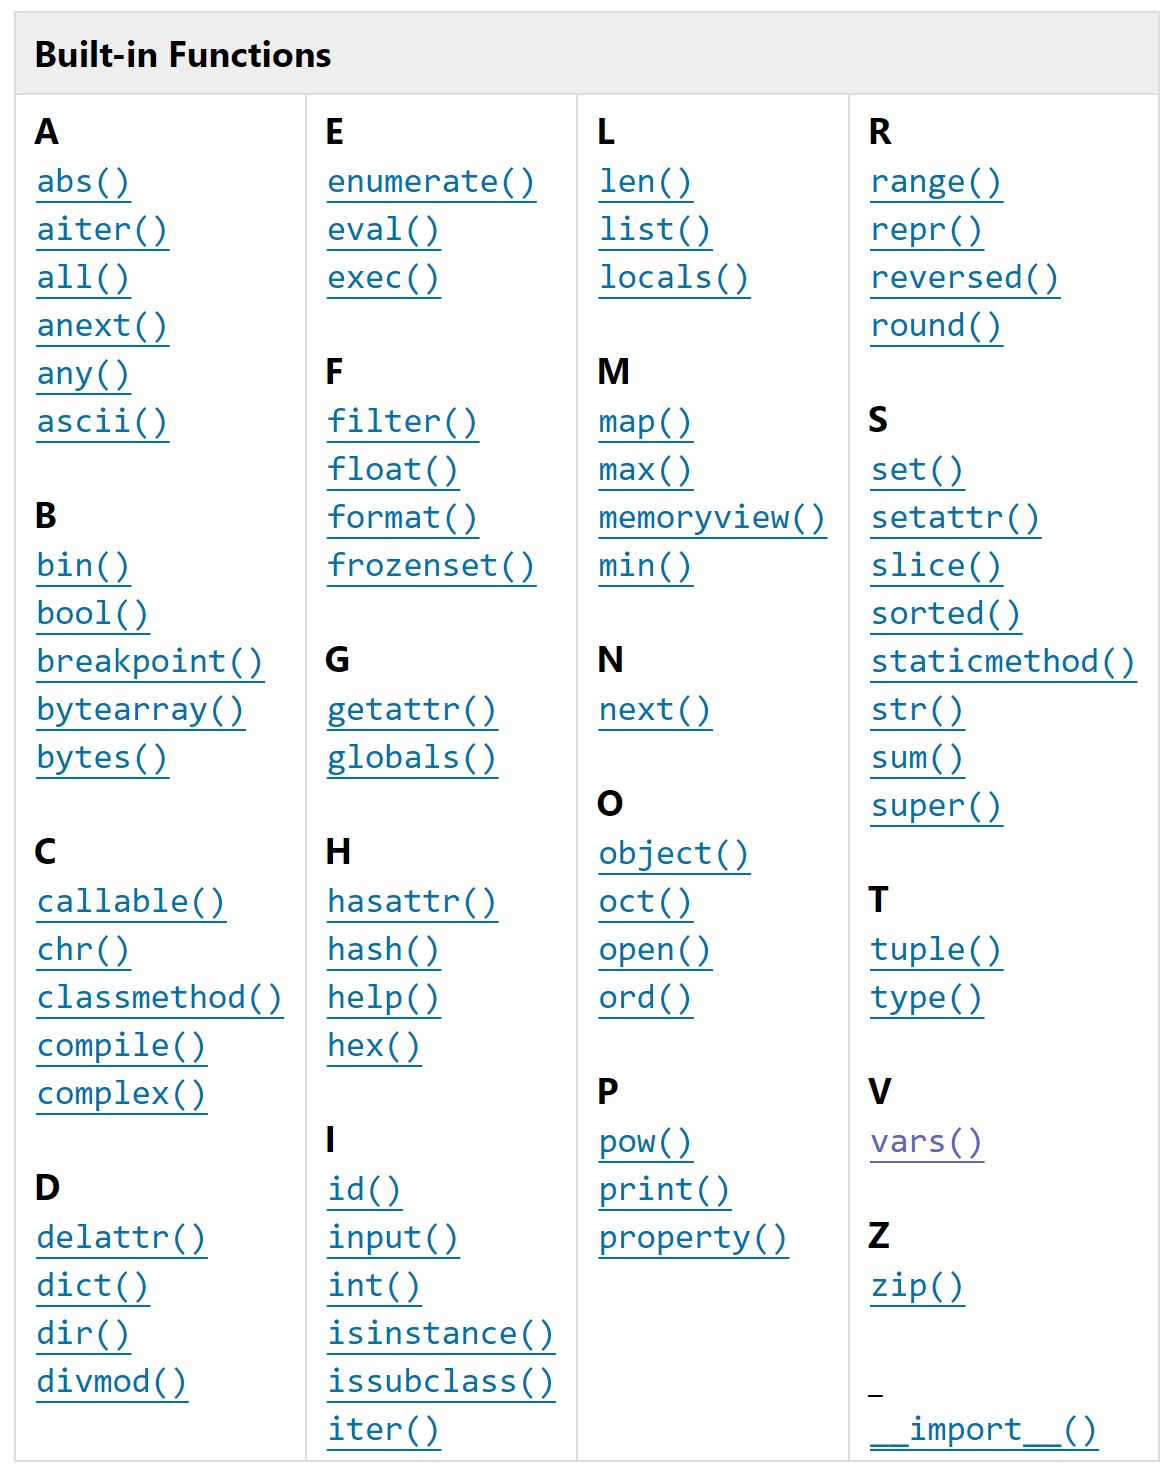
\includegraphics[width=0.6\textwidth]{images/built_in.JPG}
    \caption{Built-in Functions}
    \label{fig:misc-1}
\end{figure}

The \texttt{len()} function in Python is a built-in function that returns the length of an object. It's a versatile and commonly used tool that provides a convenient way to determine the number of elements in various data structures, such as strings, lists, tuples, dictionaries, and more.

\begin{codebox}
\begin{minted}{python}
# Example use of len() with a list
my_list = [1, 2, 3, 4, 5]
list_length = len(my_list)
print("Length of the list:", list_length)

# Example use of len() with a string
my_string = "Hello, World!"
print("Number of charactersin the string:", len(my_string))
\end{minted}
\end{codebox}

\newpage
\subsubsection{Map, Filter and Reduce}
The \texttt{map()}, \texttt{filter()}, and \texttt{reduce()} functions are powerful tools in functional programming, allowing for concise and efficient data transformations and computations over iterables. They help streamline code and make it more expressive by abstracting away common patterns of iteration and computation.
\begin{itemize}
    \item \textbf{\texttt{map()}}
    \begin{itemize}
        \item The \texttt{map()} function applies a specified function to each item in an iterable (such as a list) and returns a new iterator containing the results.
        \item Syntax: \texttt{map(function, iterable)}
        \item Example:
\begin{codebox}
\begin{minted}{python}
numbers = [1, 2, 3, 4, 5]
doubled = map(lambda x: x * 2, numbers)
print(list(doubled))  # Output: [2, 4, 6, 8, 10]
\end{minted}
\end{codebox}
        \item In this example, the \texttt{lambda x: x * 2} function is applied to each item in the \texttt{numbers} list, doubling each value.
    \end{itemize}
    
    \item \textbf{\texttt{filter()}}
    \begin{itemize}
        \item The \texttt{filter()} function constructs an iterator from elements of an iterable (such as a list) for which a specified function returns \texttt{True}.
        \item Syntax: \texttt{filter(function, iterable)}
        \item Example:
\begin{codebox}
\begin{minted}{python}
numbers = [1, 2, 3, 4, 5]
evens = filter(lambda x: x % 2 == 0, numbers)
print(list(evens))  # Output: [2, 4]
\end{minted}
\end{codebox}
        \item In this example, the \texttt{lambda x: x \% 2 == 0} function filters out only the even numbers from the \texttt{numbers} list.
    \end{itemize}
    
    \item \textbf{\texttt{reduce()}}
    \begin{itemize}
        \item The \texttt{reduce()} function is used to apply a rolling computation to sequential pairs of values in an iterable, producing a single accumulated result.
        \item Syntax: \texttt{reduce(function, iterable[, initializer])}
        \item Example:
\begin{codebox}
\begin{minted}{python}
from functools import reduce

numbers = [1, 2, 3, 4, 5]
total = reduce(lambda x, y: x + y, numbers)
print(total)  # Output: 15
\end{minted}
\end{codebox}
        \item In this example, the \texttt{lambda x, y: x + y} function is applied cumulatively to the items of the \texttt{numbers} list, resulting in the sum of all elements.
        \item In Python 3, the \texttt{reduce()} function is available in the \texttt{functools} module, so you do need to import it if you want to use \texttt{reduce()}. However, in Python 2, \texttt{reduce()} was a built-in function and didn't require an import.

    \end{itemize}
\end{itemize}

\newpage
\subsubsection{Iterator Functions}
Iterators are objects that implement the iterator protocol, which consists of two methods: \texttt{\_\_iter\_\_()} and \texttt{\_\_next\_\_()}. Iterators are used to iterate over a sequence of elements, such as lists, tuples, dictionaries, and custom objects.

\begin{itemize}
    \item \texttt{\_\_iter\_\_()}: This method returns the iterator object itself. It's called when you create an iterator using the \texttt{iter()} function or when an iterator is requested implicitly, such as in a \texttt{for} loop.
    
    \item \texttt{\_\_next\_\_()}: This method returns the next item from the iterator. It's called repeatedly to retrieve successive items from the iterator. When there are no more items to return, it raises a \texttt{StopIteration} exception.
\end{itemize}

\begin{codebox}
\begin{minted}{python}
class MyIterator:
    def __init__(self, limit):
        self.limit = limit
        self.current = 0

    def __iter__(self):
        return self

    def __next__(self):
        if self.current < self.limit:
            value = self.current
            self.current += 1
            return value
        else:
            raise StopIteration()
            

# Using the custom iterator
iterator = MyIterator(5)
for item in iterator:
    print(item)
\end{minted}
\end{codebox}

This example demonstrates how to create a simple custom iterator in Python that follows the iterator protocol. It generates values lazily, allowing for efficient memory usage, especially when dealing with large datasets or infinite sequences. The \texttt{\_\_iter\_\_()} method is called when an object is used in an iterable context, such as in a for loop, to obtain an iterator for the object. Iterators support the \texttt{next()} function, which is used to retrieve the next item from the iterator.\\

\newpage
Several Python built-in functions return iterators or objects that can be iterated over. Some of the most commonly used ones include:

\begin{itemize}
    \item \textbf{\texttt{iter()}}: This built-in function returns an iterator object for the given iterable. If the object is already an iterator, it returns itself. Otherwise, it calls the \texttt{\_\_iter\_\_()} method of the object to obtain an iterator.
    
    \item \textbf{\texttt{enumerate()}}: Returns an iterator that yields tuples containing a count (starting from zero by default) and the values obtained from iterating over the iterable.
    
    \item \textbf{\texttt{map()}}: Applies a given function to each item of an iterable (like a list or tuple) and returns an iterator that yields the results.
    
    \item \textbf{\texttt{filter()}}: Constructs an iterator from those elements of the iterable for which the function returns \texttt{True}.
    
    \item \textbf{File objects}: When reading from a file in Python, file objects return iterators over lines of the file. For example, when using a \texttt{for} loop to iterate over lines in a file, each iteration returns the next line from the file.
    
    \item \textbf{\texttt{range()}}: In Python 3, \texttt{range()} returns a range object that behaves like an iterator. It generates numbers within a specified range on demand rather than storing them all in memory.
\end{itemize}

The \texttt{iter()} function is used to obtain iterators from different types of iterables: a list, a custom callable, and a file object. Once you have an iterator, you can iterate over it using a \texttt{for} loop, use it with other functions that accept iterators, or manually call \texttt{next()} on it to retrieve the next element.

\begin{codebox}
\begin{minted}{python}
my_list = [1, 2, 3, 4, 5]
my_iterator = iter(my_list)
# Print the first element of the list
print(next(my_iterator))

# Iterate over the remaining elements using a for loop
for i in my_iterator:
    print(i)
\end{minted}
\end{codebox}

The \texttt{enumerate()} function is used to iterate over a sequence (such as a list, tuple, or string) while also tracking the index of each item. It returns an iterator that yields tuples containing both the index and the value of each item in the sequence.
\begin{codebox}
\begin{minted}{python}
my_list = ['apple', 'banana', 'cherry']

for index, value in enumerate(my_list):
    print(f"Index: {index}, Value: {value}")
\end{minted}
\end{codebox}

A range object is not technically an iterator, but it behaves similarly to one. The \texttt{range} object itself does \textbf{not} have a \texttt{next()} method.
\begin{codebox}
\begin{minted}{python}
# Create a range object with range(start, stop, step)
my_range = range(10, 0, -2)

# Print each number generated by the range object using next()
for i in my_range:
    print(i) # 10, 8, 6, 4, 2
\end{minted}
\end{codebox}

\newpage
\subsubsection{Generator Functions}
Generators are a \textit{special type of iterator} created using generator functions or generator expressions. Iterators are a general concept in Python for objects that can be iterated over, while generators are a specific implementation of iterators that provide a concise and efficient way to generate values lazily using generator functions or expressions. Generators are a powerful tool for working with iterators, especially when dealing with large datasets or when generating sequences dynamically.\\

Generator functions use the \texttt{yield} keyword to produce a series of values lazily, allowing for efficient memory usage and enabling the processing of large datasets or infinite sequences. Generators functions pause and resume their execution, allowing them to produce a sequence of values over time, rather than computing them all at once and storing them in memory.\\

When you use \texttt{yield} in a function, it turns that function into a generator. When the function is called, it doesn't execute immediately; instead, it returns a generator object. When you iterate over this generator object using a loop or other iteration constructs, the function starts executing, and when it encounters a \texttt{yield} statement, it temporarily suspends its execution and returns the value specified by yield. The next time you iterate over the generator, it resumes execution from where it left off.

\begin{codebox}
\begin{minted}{python}
def my_generator():
    yield 1
    yield 2
    yield 3

# Using the generator
gen = my_generator()
print(next(gen))  # Output: 1
print(next(gen))  # Output: 2
print(next(gen))  # Output: 3
# print(next(gen))  # Would raise StopIteration error
\end{minted}
\end{codebox}

\begin{codebox}
\begin{minted}{python}
def fibonacci():
    a, b = 0, 1
    while True:
        yield a
        a, b = b, a + b

# Create a Fibonacci generator
fib_gen = fibonacci()

# Print the first 10 Fibonacci numbers
print("First 10 Fibonacci numbers:")
for _ in range(10):
    print(next(fib_gen))
\end{minted}
\end{codebox}
The key here is that the tuple texttt{(b, a + b)} is created before any assignment occurs, so \texttt{a} is assigned the value of \texttt{b} and \texttt{b} is assigned the sum of the old values of \texttt{a} and \texttt{b}. This allows for a simultaneous update of both variables without needing a temporary variable.


\newpage
\subsubsection{Lambda Functions}
Lambda functions, also known as \textbf{anonymous functions}, are small, inline functions that are defined using the \texttt{lambda} keyword. Unlike regular functions defined using the \texttt{def} keyword, lambda functions are single-expression functions that can be created quickly without needing a formal \texttt{def} statement.

\begin{codebox}
\begin{minted}{python}
Adding two numbers
add = lambda x, y: x + y
print(add(3, 5))  # Output: 8

# Squaring a number
square = lambda x: x ** 2
print(square(4))  # Output: 16

# Checking if a number is even
is_even = lambda x: x % 2 == 0
print(is_even(5))  # Output: False
print(is_even(6))  # Output: True
\end{minted}
\end{codebox}

To create an iterator that yields only the even numbers from a given list, the \texttt{filter()} function is utilized along with a lambda function. The \texttt{filter()} function takes two arguments: the first argument is the lambda function that defines the condition for filtering, and the second argument is the iterable from which elements are filtered. In this case, the lambda function checks if a number \texttt{x} is even by performing the modulo operation \texttt{\% 2} and comparing the result to 0. The \texttt{filter()} function then returns an iterator that yields only those elements from the input iterable for which the lambda function returns \texttt{True}. Finally, the filtered iterator is iterated over to print the even numbers.

\begin{codebox}
\begin{minted}{python}
# Define a list of numbers
numbers = [1, 2, 3, 4, 5, 6, 7, 8, 9, 10]

# Use filter() with a lambda function
even_numbers_iterator = filter(lambda x: x % 2 == 0, numbers)

# Iterate over the filtered iterator and print the even numbers
print("Even numbers:")
for num in even_numbers_iterator:
    print(num)
\end{minted}
\end{codebox}

%\begin{codebox}
%\begin{minted}{python}
%
%\end{minted}
%\end{codebox}




